\documentclass[12pt]{extarticle}

\usepackage[]{cite}
\usepackage{cmap}
\usepackage[T2A]{fontenc}
\usepackage[utf8]{inputenc}
\usepackage[english, russian]{babel}

% \usepackage{jmlda}
\newcommand{\hdir}{.}
\usepackage{amsmath, amsfonts,amssymb,mathrsfs}
\usepackage{graphicx}
\usepackage{minted}
\usepackage{hyperref}
\usepackage{mathtools}
\usepackage{tocloft}
\usepackage[linesnumbered,boxed]{algorithm2e}
% \usepackage{algorithm}
% \usepackage{algpseudocode}
% \usepackage[usenames]{color}
% \usepackage{colortbl}


\usepackage{graphicx, epsfig}
\usepackage{subfig}
\usepackage{color}

\usepackage{wrapfig}
\usepackage{float}
\usepackage{subfloat}
\usepackage{caption}
\usepackage{multirow}



\newtheorem{theorem}{Теорема}
\newtheorem{lemma}[theorem]{Лемма}
\newtheorem{definition}{Определение}
\newtheorem{remark}{Замечание}
\newenvironment{Proof} % имя окружения
    {\par\noindent{\bf Доказательство.}} % команды для \begin
    {\hfill$\scriptstyle\blacksquare$} % команды для \end

\DeclareMathOperator*{\argmax}{arg\,max}
\DeclareMathOperator*{\argmin}{arg\,min}
\newcommand{\Domain}{\mathcal{D}}
\newcommand{\supp}{\mathrm{supp}}
\newcommand{\diag}{\mathrm{diag}}
\newcommand{\bfw}{\mathbf{w}}
\newcommand{\bfv}{\mathbf{v}}
\newcommand{\bfx}{\mathbf{x}}
\newcommand{\bfz}{\mathbf{z}}
\newcommand{\bfX}{\mathbf{X}}
\newcommand{\bfy}{\mathbf{y}}
\newcommand{\bfb}{\mathbf{b}}
\newcommand{\bbr}{\mathbb{R}}
\newcommand{\bsigma}{\boldsymbol\Sigma}
\newcommand{\expectation}{\mathbb{E}}
\newcommand{\ceil}[1]{\lceil #1 \rceil}

\def\BibAuthor#1{\ruseng{\textit{#1}}}
\def\BibTitle#1{\ruseng{\textrm{#1}}}
\def\BibJournal#1{\ruseng{\textrm{#1}}{\textsl{#1}}}
\def\BibUrl#1{{\small\url{#1}}}
\def\BibHttp#1{{\small\url{http://#1}}}
\def\BibFtp#1{{\small\url{ftp://#1}}}
\def\BibDoi#1{doi:~{\small\url{http://dx.doi.org/#1}}}
\def\typeBibItem{\small\sloppy}


\textheight=22cm % высота текста
\textwidth=16cm % ширина текста
\oddsidemargin=0pt % отступ от левого края
\topmargin=-1.5cm % отступ от верхнего края
\parindent=24pt % абзацный отступ
\parskip=5pt % интервал между абзацами
\tolerance=2000 % терпимость к "жидким" строкам
\flushbottom % выравнивание высоты страниц

\begin{document}
% \thispagestyle{empty}
% \begin{center}
%     \sc
%         «Московский физико-технический институт \rm{(национальный исследовательский университет)}»\\
%         Физтех-школа прикладной математики и информатики\\
%         Кафедра <<Интеллектуальные системы>>
%         %\\        при Вычислительном центре им. А. А. Дородницына РАН
%         \\[35mm]
%     \rm\large
%         Шокоров Вячеслав Александрович\\[10mm]
%     \bf\Large
% 		Оценка параметров вероятностной модели в задаче доменной адаптации\\[10mm]
%     \rm\normalsize
%         03.03.01 -- Прикладные математика и физика\\[10mm]
%     \sc
%         Выпускная квалификационная работа бакалавра\\[10mm]
% \end{center}
% \hfill\parbox{85mm}{
%     \begin{flushleft}
%     \bf
%         Научный руководитель:\\
%     \rm
%         д.ф.-м.н. Стрижов Вадим Викторович\\[3.9cm]
%     \end{flushleft}
% }
% \begin{center}
%     Москва\\
%     2021
% \end{center}

% \newpage
\tableofcontents
\newpage

\begin{abstract}
Методы классического машинного обучения хорошо работают, когда обучающие и тестовые данные взяты из одного и того же распределения. Однако во многих ситуациях у нас могут быть только обучающие данные для исходного домена, задача заключается в обучении модели, которая будет хорошо работать на целевом домене с другим распределением. Какими функциями сходства распределения и каким методом мы можем адаптировать модель, обученный в исходном домене для использования на целевом домене? Интуитивно понятно, что хорошее представление признаков является решающим фактором успеха адаптации домена. 

Предлагаемый подход вдохновлен теорией адаптации домена, предполагающей, что для достижения эффективной трансформации домена, функция преобразования должна делать домены неразличимыми, это достигается максимизацией функции сходства. Подход реализует эту идею в контексте архитектур нейронных сетей.
 \\
\bigskip
\noindent

\textbf{Ключевые слова}: \emph {доменная адаптация, нейронная сеть, GAN, WGAN, функция сходства Адуенко. А.\ А.}
\end{abstract}
\newpage

%данные поля заполняются редакцией журнала
% \doi{10.21469/22233792}
% \receivedRus{01.01.2017}
% \receivedEng{January 01, 2017}

% \maketitle

% \cftchapterprecistoc




\section{Введение}



% \addcontentsline{toc}{section}{\protect\numberline{}Введение}




\subsection{Введение}

В данной раб решается задача доменной адаптации. Цель этой адаптации заключается в обучении модели на данных из домена-источника так, чтобы она показывала сравнимое качество на целевом домене. Например, домен-источник может представлять собой синтетические данные, которые можно сгенерировать без значительных затрат и которые будут иметь хорошую, качественную разметку, а целевой домен~--- фотографии пользователей. Тогда задача доменной адаптации заключается в обучении модели на синтетических данных, которая будет хорошо работать с «реальными» объектами. 

\begin{figure}[H]
        \centering
        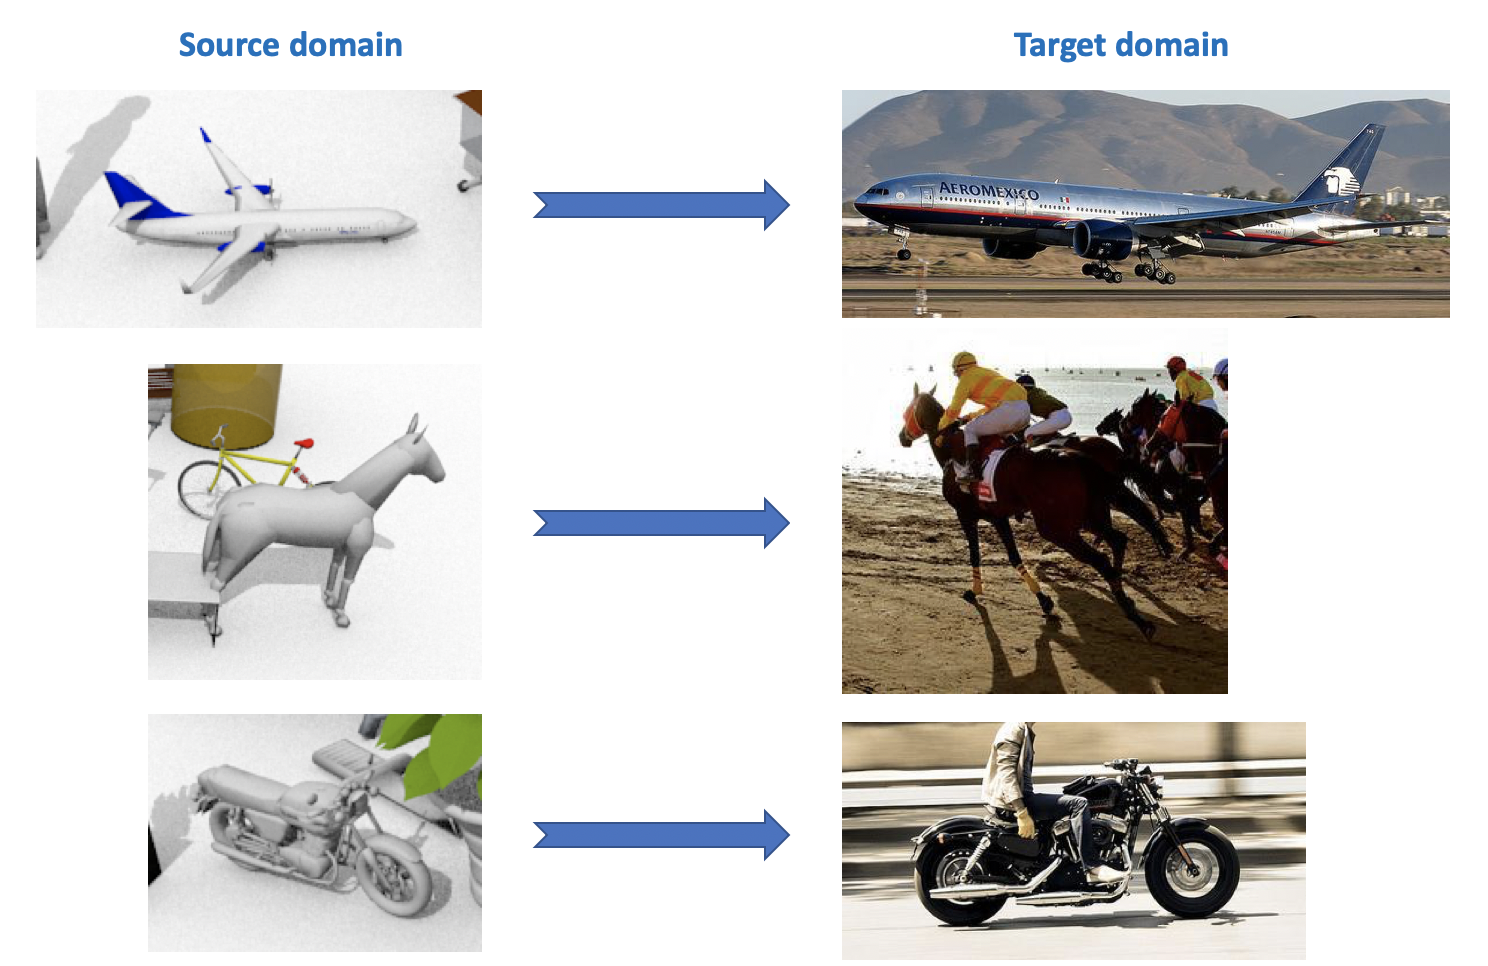
\includegraphics[width=0.8\textwidth]{pictures/from_source_to_target.png}
        
        \caption{Примеры задачи применения адаптации доменов. Изображения взяты из датасета VisDA, который  используется в конкурсе Visual Domain Adaptation Challenge.}
        % \label{example:1}
\end{figure}

Данную задачу предлагается решить через построение функции преобразования одного домена в другой, максимизируя функцию сходства. Мы выдвигаем и проверяем на вычислительном эксперименте гипотезу о том, что, если распределения доменов схожи, то и веса моделей обученных на них будут совпадать. Это утверждение является мотивацией подхода.

Исследуется проблема построения и анализа вероятностного пространства параметров этого преобразования. Проблема усложнена тем, что домены могут принадлежать непересекающимся или слабо пересекающихся пространствам. Очевидно, что в таком случае, без использования функции преобразования, классические подходы машинного обучения, когда обучается модель на исходном домене и применяется к целевому домену, не имеет смысла. Случай частично-ортогональных признаковых пространств доменов возможен, например, когда рассматриваются товары в магазине. Есть наблюдаемые параметры этих объектов (для карандашей - цвет грифеля и его мягкость, для книг~--- количество страниц и тип переплета), множество наблюдаемых параметров может как пересекаться (общий параметр для карандашей и книг~--- цена), так и не пересекаться (цвет грифеля, количество страниц). Подходы обучения без учителя также дают недостаточное качество, так как не используют информацию, которую можно получить из первого домена.

    
\begin{definition}
Доменом называется априорное распределение признакового описания объектов.
\end{definition}

\begin{definition}
Функция $f$ называется функцией преобразования домена $\Domain_1$ в домен $\Domain_2$, если $f: \supp(\Domain_1) \to \supp(\Domain_2)$
\end{definition}



\begin{figure}[H]
        \centering
        \subfloat[\centering исходная выборка]{{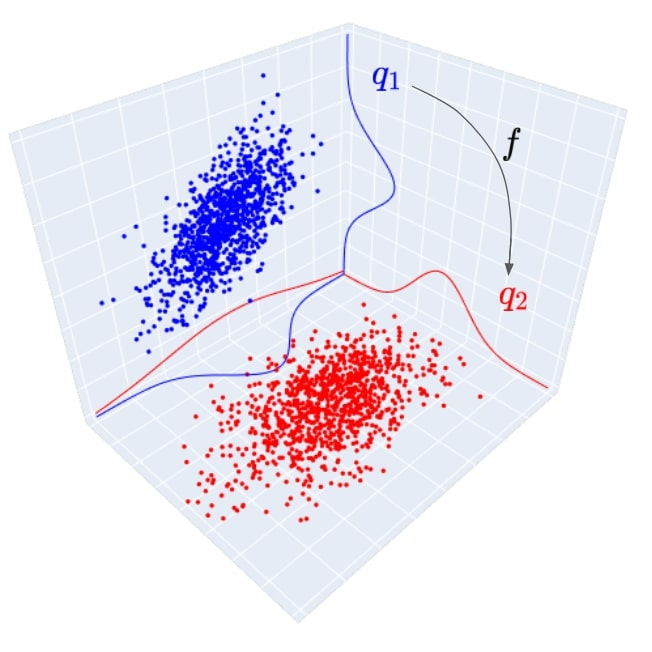
\includegraphics[width=0.4\textwidth]{pictures/2_margin_dist_before_annotated.jpg} }}
        \qquad
        \subfloat[\centering преобразованная выборка]{{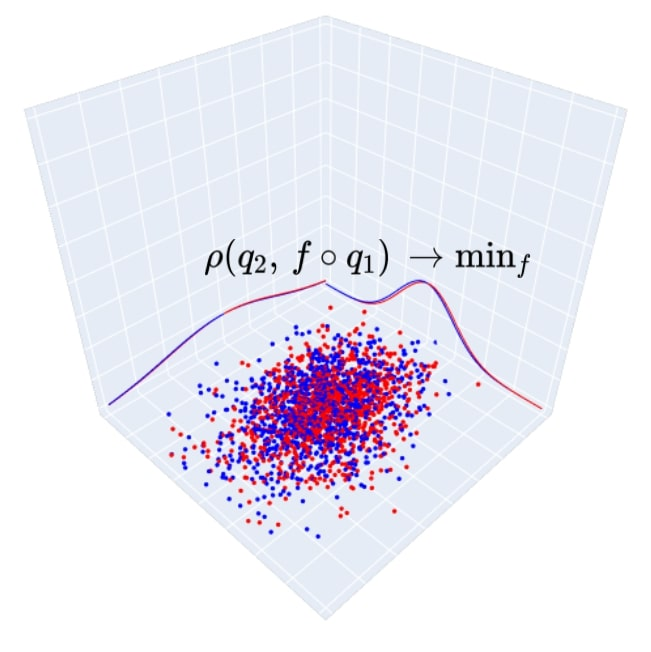
\includegraphics[width=0.4\textwidth]{pictures/2_margin_dist_after_annotated.jpg} }}
        
        \caption{Упрощенный пример-визуализация применения предлагаемого подхода. (a) Два домена, первый (целевой, синий) описывается признаками из пространства z-x, второй (исходный, красный) из  пространства x-y. Для каждого домена задано распределение. (b) для первого домена применена функция преобразования. Параметры преобразования находятся при решении задачи минимизации функции сходства, которая сравнивает второй домен и преобразованный первый.}
        % \label{example:1}
    \end{figure}
    
\newpage

\subsection{Обзор литературы}

Существует большой набор методов доменной адаптации. Данная работа посвящена применению Adversarial-Based подходов. Эти подходы используют состязательную функцию ошибки, которая впервые появилась в GAN'ах.

Ключевой особенностью методов из этого семейства является обучение нейронной сети с инвариантным по отношению к исходному и целевому доменам векторным представлением. Тогда обученную на размеченном исходном домене сеть можно будет использовать на целевом домене, в идеале — практически без потери качества классификации.


В работе \cite{DANN} предлагается применение трех моделей: основной сети, с помощью которой получается векторное представление , ''головы'', отвечающей за классификацию на исходном домене и ''головы'', которая обучается отличать данные из исходного домен от целевого. Особенностью данного подхода является применение Gradient reversal layer при обратном распространении ошибки в обучении для ''головы'', отвечающей за домены. Этот добавочный слой умножает проходящий через него градиент на негативную константу, увеличивая функцию ошибки связанную с доменном. Этим добиваются того, что распределения векторных представлений на обоих доменах становятся близки.


В подходе под названием Adversarial Discriminative Domain Adaptation (ADDA), описанном в \cite{ADDA}, применяется разделение сети для исходного домена и сети для целевого домена. Суть ADDA заключается в том, что мы сначала обучаем хороший классификатор на размеченном исходном домене, а затем с помощью состязательного-обучения адаптируем так, чтобы векторные представления классификатора на обоих доменах были близки. 


\section{Теоретическая часть}
\subsection{Постановка задачи}

В качестве функции преобразования будем брать нейронную сеть с параметрами $\theta_f$.
    
\begin{definition}
    \textit{Оптимальной функцией преобразования} домена $\mathcal{D}_1$ в домен $\mathcal{D}_2$ относительно функции сходства $s$ назовем функцию $f_s(\cdot, \hat{\theta}_f)_s$:
    \begin{equation}
        \label{opt_transorm_f}
        \hat{\theta}_f = \argmax_{\theta_f} s\Big( \Domain_2,  p(f(x, \theta_f), x \sim \Domain_1)\Big)
    \end{equation}
Для краткости будем обозначать $\hat{f}_s(\cdot) = f_s(\cdot, \hat{\theta}_f)_s$.
\end{definition}


\subsubsection{Постановка задачи для функции предложенной Адуенко А. А.}

В работе \cite{Aduenko_article} Адуенко А. А. ввел функцию сходства:
\begin{definition}
    Назовем функцией сходства $s_0$ пары распределений $g_1 : \bbr^n \to \bbr^{+}, g_2 : \bbr^n \to \bbr^{+}$, определенных на одном пространстве, функцию вида
    
    $$s_0(g_1, g_2) = \frac{\int g_1(\bfx)g_2(\bfx) d\bfx}{\max_{\bfb\in\bbr^n} \int g_1(\bfz)g_2 (\bfz - \bfb)d\bfz}$$ 
\end{definition}


Перед началом решения задачи и поиском параметры функции преобразования необходимо проверить, что функция Адуенко является критерием совпадения распределений, т.е. верно ли, что:

$$s_0(g_1, g_2) = 1 \xLeftrightarrow{?}  g_1 \equiv g_2$$
Либо в для последовательности распределений $\{g^k_2\}^\infty_{k=1}$:

\begin{equation}
    \label{aduenko_criteria}
    s_0(g_1, g^k_2) \xrightarrow[]{k\to \infty} 1 \xLeftrightarrow{?}  g^k_2 \xrightarrow[]{k\to \infty} g_1.
\end{equation}

\begin{theorem}
\label{th:Aduenko_necessary} 
Пусть дана пара распределений $g_1(\bfx): \mathbb{R}^{n_1} \to \mathbb{R}^+,$ $g_2(\bfx): \mathbb{R}^{n_2} \to \mathbb{R}^+,$ где $n_1, n_2 > 0$. Тогда для некоторой последовательности параметрических линейных преобразований $\{f^k_{\theta}\}^\infty_{k=1}$, такой что $\|g_1 - f^k_\theta\circ g_2\| \to 0$, верно:
$$ s_0(g_1,f^k_\theta\circ g_2) \to 1$$
\end{theorem}

\begin{lemma}
\label{lem:Aduenko_necessary} 
Пусть дано распределение $g_1(\bfx): \bbr^{n} \to \bbr^+$ и последовательность распределений $g^k_2(\bfx): \bbr^{n} \to \mathbb{R}^+$. 
Тогда, если $\|g_1 - g^k_2\| \to 0$, верно:
$$ s_0(g_1,f^k_\theta\circ g_2) \to 1$$
\end{lemma}

\begin{Proof}%[Доказательство]

Зададим $g^k_\Delta = g^k_2 - g_1$, тогда из $\|g^k_\Delta\| \to 0$ следует, что $\int g^k_\Delta \to 0$.

\begin{multline}
    \label{lem:Aduenko_necessary_1}
    s_0(g_1, g_1 + g^k_\Delta) = \frac{\int g_1(\bfx) (g_1 + g^k_\Delta)(\bfx)d\bfx}{\max_{\bfb} \int g_1(\bfz) (g_1 + g^k_\Delta)(\bfz + \bfb) d\bfz} = \\ \frac{\int g^2_1(\bfx)d\bfx + \int g_1(\bfx) g^k_\Delta(\bfx)d\bfx }{\max_{\bfb} \Big[ \int g_1(\bfz) g_1(\bfz + \bfb) d\bfz + \int g_1(\bfz) g^k_\Delta(\bfz + \bfb) d\bfz \Big]} \geq \\ \frac{\int g^2_1(\bfx)d\bfx + \int g_1(\bfx) g^k_\Delta(\bfx)d\bfx }{\max_{\bfb} \int g_1(\bfz) g_1(\bfz + \bfb) d\bfz + \max_{\bfb'} \int g_1(\bfz) g^k_\Delta(\bfz + \bfb') d\bfz }
\end{multline}
Рассмотрим знаменатель полученного выражения. Из неравенства Коши-Буняковского:

$$ \int g_1(\bfz)g_1(\bfz - \bfb)d\bfz \leq \sqrt{\int g^2_1(\bfz)d\bfz} \sqrt{\int g^2_1(\bfx - \bfb)d\bfx} = \int g^2_1(\bfx)d\bfx,$$
Причем при $\bfb = \mathbf{0}$ неравенство обращается в равенство. Подставляя данное выражение в \eqref{lem:Aduenko_necessary_1}, получаем:

$$ s_0(g_1, g_1 + g^k_\Delta) \geq \frac{\int g^2_1(\bfx)d\bfx + \int g_1(\bfx) g^k_\Delta(\bfx)d\bfx }{ \int g^2_1(\bfz) d\bfz + \max_{\bfb} \int g_1(\bfz) g^k_\Delta(\bfz + \bfb) d\bfz } \to 1, \text{ при } k\to \infty$$
Откуда следует доказываемое утверждение.

\end{Proof}

Отметим, что теорема \ref{th:Aduenko_necessary} является частным случаем леммы \ref{lem:Aduenko_necessary}.

\begin{theorem}
\label{th:Aduenko_not_sufficient} 
Пусть дана пара распределений $g_1(\bfx): \mathbb{R}^{n_1} \to \mathbb{R}^+,$ $g_2(\bfx): \mathbb{R}^{n_2} \to \mathbb{R}^+,$ где $n_1, n_2 > 0$. Тогда существует некоторая последовательность параметрических линейных преобразований $\{f^k_{\theta}\}^\infty_{k=1}$, такая что $s_0(g_1, f^k_\theta\circ g_2) \to 1$, и для нее не верно:
$$\|g_1 - f^k_\theta\circ g_2\| \to 0$$
\end{theorem}


\begin{lemma}
\label{lem:Aduenko_not_sufficient} 
Для линейного преобразование $f^k_{\theta}(x)$, которое имеет вид $x/k + b$, где $k\in \mathbb{N}_{+}, \bfb = \argmax_\bfx g_2(\bfx), \ \bfb \in \bbr^{n_2}$ Выполняются следующие свойства:

\begin{equation}
    \label{Ad_n_suf_1}
    \forall a > 0, f^k_\theta\circ g_2(\cdot) |_A \to U(A), \text{ где } A = \{\bfx : \|\bfx\| \leq a\}
\end{equation}

\begin{equation}
    \label{Ad_n_suf_2}
    \exists 0 \leq B < \infty, \ \exists k_0 : \forall k \geq k_0 \sup_{\{\bfx: \|\bfx\|\geq B\}} f^k_\theta\circ g_2(\bfx) \leq \sup_{\{\bfx: \|\bfx\| \leq B\}} f^k_\theta\circ g_2(\bfx),
\end{equation}
где в свойстве \eqref{Ad_n_suf_1} $f^k_\theta\circ g_2(\cdot) |_A$ есть сужение $f^k_\theta\circ g_2(\cdot)$ на множество $A$, то есть 

$$ g_2(\cdot) |_A (\bfx) = \begin{cases} 0, \text{ если } \bfx \not\in A \\ \frac{g_2(\bfx)}{\int_A g_2(\bfz) d\bfz}, \bfx \in A \end{cases} $$
Сходимость в свойстве \eqref{Ad_n_suf_1} понимается равномерная, то есть 

$$g_2(\cdot) \to U(A) \Leftrightarrow \sup_{\bfx \in A} \Big|g_2(\bfx) - 1/|A|\Big| \to 0, \text{ где } k \to \infty. $$
\end{lemma}

\begin{Proof}

С учетом того, что интеграл функции распределения по $\bbr^{n_2}$ должен равняться 1, получаем, что последовательность распределений имеет вид: 

$$f^k_{\theta}\circ g_2(\bfx) = g_2\Big(\frac{\bfx}{k} + \bfb\Big)\Big/
k$$ 
Проверим выполнимость свойства \eqref{Ad_n_suf_1}. Так как $\bfb$ является точкой максимума неотрицательной и ненулевой функции, следовательно $g_2(\bfb) > 0$. Зафиксируем произвольные $\delta \in (0, g_2(\bfb)), a > 0$ 

Тогда существует $w_\delta$ такая, что для всех $\bfx$ лежащих внутри окрестности нуля, т.е. $\|\bfx\| < w_\delta$ верно $g_2(\bfb) - \delta \leq g_2(\bfx + \bfb) \leq g_2(\bfx)$. Отсюда, для $\forall k \geq \ceil{\frac{a}{w_\delta}}$ и $\forall \bfx \in A$ верно:

\begin{equation}
    \label{Ad_n_suf_3}
    \frac{1}{k} \Big (g_2(\bfb) - \delta\Big) \leq \frac{1}{k} g_2\Big(\frac{\bfx}{k} + \bfb\Big) \leq \frac{1}{k} g_2(\bfb)
\end{equation}
Из чего верно:

\begin{equation}
    \label{Ad_n_suf_4}
    \frac{1}{k} \Big (g_2(\bfb) - \delta\Big)|A| \leq \int_A \frac{1}{k} g_2\Big(\frac{\bfx}{k} + \bfb\Big) \leq \frac{1}{k} g_2(\bfb) |A|
\end{equation}
Далее объединяя \eqref{Ad_n_suf_3} и \eqref{Ad_n_suf_4} получаем:

\begin{equation*}
    \frac{\frac{1}{k} \Big (g_2(\bfb) - \delta\Big)}{\frac{1}{k} g_2(\bfb) |A|} \leq \frac{1}{k} g_2\Big(\frac{\bfx}{k} + \bfb\Big)\Big|_A = \frac{\frac{1}{k} g_2\Big(\frac{\bfx}{k} + \bfb\Big)}{\int_A \frac{1}{k} g_2\Big(\frac{\bfx}{k} + \bfb\Big)} \leq \frac{\frac{1}{k} g_2(\bfb)}{\frac{1}{k} \Big (g_2(\bfb) - \delta\Big)|A|}
\end{equation*}
Если упростить и вычесть $1/|A|$ из каждой части получим:

\begin{equation}
    \label{Ad_n_suf_5}
    \frac{ - \delta}{g_2(\bfb) |A|} \leq \frac{1}{k} g_2\Big(\frac{\bfx}{k} + \bfb\Big)\Big|_A - \frac{1}{|A|} \leq \frac{\delta}{(g_2(\bfb) - \delta)|A|}
\end{equation}
Тогда в силу произвольности $\delta$ получаем равномерную сходимость сужения элементов последовательности распределений на множество $A$ к $U(A)$, тем самым доказываем выполнения первого свойства \eqref{Ad_n_suf_1}.

Выполнение второго свойства очевидно, так как $0$ - точка максимума и увеличение $k$ сдвигает ее. 

\begin{figure}[H]\center
    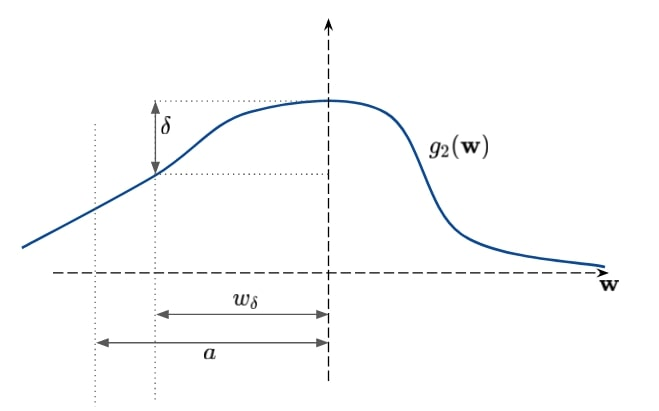
\includegraphics[width=0.7\textwidth]{pictures/visual_idea_with_delta.jpg}
    \caption{Поясняющий рисунок к доказательству леммы. При увеличении $k$ получается, что распределение "растягивается" от нуля, а окрестность, в которой значение функции отличается только на максимального значение, постепенно выходит за $A$.}
    \label{fig_1}
\end{figure}
    
\end{Proof}



\bigskip

\begin{Proof}\textbf{ Теоремы \ref{th:Aduenko_not_sufficient}.}

Для доказательства теоремы построим последовательность преобразований описанную в Лемме \ref{lem:Aduenko_not_sufficient}. Обозначим $g_2\Big(\frac{\bfx}{k} + \bfb\Big)$ как $g^k_2(\bfx)$. Таким образом требуется показать, что 

$$\frac{ \int g_1(\bfx)g^k_2(\bfx)d\bfx}{\max_\bfb \int g_1(\bfz)g^k_2(\bfz - \bfb)d\bfz} \to 1 \text{ при } k \to \infty$$
Обозначим $Q_a = \{\bfx : \|\bfx\| \geq a\}, R_a = \{\bfx : \|\bfx\| \leq a\}$. Из свойства \eqref{Ad_n_suf_2} в лемме \ref{lem:Aduenko_not_sufficient} имеем:

$$\exists 0 \leq B < \infty, \ \exists k_0 : \forall k \geq k_0 \ \sup_{Q_B} g^k_2(\bfx) \leq \sup_{R_B} g^k_2(\bfx).$$
Зафиксируем произвольное $\epsilon > 0$. Определим $B_\epsilon$ так, что 

$$ \int_{\{\bfx : \|\bfx \| \geq B_\epsilon\}} g_1(\bfz)d\bfz < \epsilon.$$
Определим $\Tilde{B} = \max(B, B_\epsilon)$. Зафиксируем также $\delta > 0$. Из свойства \eqref{Ad_n_suf_1} в лемме \ref{lem:Aduenko_not_sufficient} имеем:

$$\exists k_\delta : \forall k \geq k_\delta \  \frac{\sup_{R_{\Tilde{B}}}g^k_2(\bfx)}{\inf_{R_{\Tilde{B}}}g^k_2(\bfx)} \leq 1 + \delta.$$
Определим $\Tilde{k} = \max(k_\delta, k_0)$. Тогда для $k \geq \Tilde{k}$ имеем

\begin{multline}
    \label{Ad_n_suf_6}
    \int g_1(\bfx)g^k_2(\bfx)d\bfx \geq \int_{\{\bfx: \|\bfx\|\leq B\}} g_1(\bfx)g^k_2(\bfx)d\bfx \geq \\ \inf_{\{\bfx: \|\bfx\|\leq B\}} g^k_2(\bfx) \int_{\{\bfz: \|\bfz\|\leq B\}} g_1(\bfz)d\bfz \geq (1 - \epsilon) \inf_{R_B} g^k_2(\bfx) \geq \\ (1 - \epsilon)(1 - \delta) \sup_{R_B} g^k_2 (\bfx). 
\end{multline}
Аналогично для знаменателя выражения для $s_0$ с учетом свойства \eqref{Ad_n_suf_2} 

\begin{equation}
    \label{Ad_n_suf_7}
    \forall \bfb \int g_1(\bfz)g^k_2(\bfz - \bfb)d\bfz \leq \sup_{\bfz}g^k_2(\bfz) = \sup_{R_B}g^k_2(\bfz).
\end{equation}
Тогда из \eqref{Ad_n_suf_6} и \eqref{Ad_n_suf_7} получаем:

$$ \forall k \geq \Tilde{k} : s_0(g_1, g^k_2) \geq (1 - \epsilon)(1 - \delta). $$
С учетом произвольности выбора $\epsilon, \delta$ получаем требуемое. Так как такое линейное преобразование "растягивает"  распределение, т.е. 

$$ \forall \bfx \ g^k_2(\bfx) \to 0, \text{ при } k \to \infty$$
Что эквивалентно тому, что:

$$ \|g^k_2\| \to 0, \text{ при } k \to \infty$$
Поэтому из условия $\|g_1 - g^k_2\| \to 0$ следует, что $g_1 \equiv 0$, что в общем случае неверно. Тем самым доказываем теорему.


\end{Proof}


Из теоремы \ref{th:Aduenko_necessary} и теоремы \ref{th:Aduenko_not_sufficient} следует, что функция Адуенко А. А. является необходимой, но недостаточной в качестве меры совпадения распределений. Т.е. не выполняется \eqref{aduenko_criteria}. Из-за чего данная функция не используется для нахождения параметров преобразования. 

\newpage
\subsubsection{Постановка задачи для дивергенция Кульбака-Лейблера}

Теперь рассмотрим дивергенцию Кульбака-Лейблера в качестве функции сходства. Для двух функций распределения $g_1, g_2$:

\begin{equation}
    \label{D_KL_intro}
    D_{KL} (g_1, g_2) = \int g_1(\bfx) \log \frac{g_1(\bfx)}{g_2(\bfx)}d\bfx = \expectation_{\bfx\sim g_1} \log g_1(\bfx) - \expectation_{\bfx\sim g_1} \log g_2(\bfx)
\end{equation}
$D_{KL}$ достигает минимума при совпадении распределений $g_1$ и $g_2$. Так же видно, что дивергенция Кульбака-Лейблера асимметрична. В тех случаях, когда $g_1(\bfx)$ близко к нулю, а $g_2(\bfx)$ значительно отличается от нуля, то получается, что $g_2$ оказывает малое влияние. Это может привести к ошибочным результатам, когда мы просто хотим измерить сходство между двумя одинаково важными распределениями.

% \textcolor{red}{\textbf{Вставить почему KL - критерий!!!}}

\begin{definition}
    Назовем функцией сходства порожденную метрикой $D$:
    \begin{equation}
        \label{sim_funk_generated_by}
        s_D (g_1 , g_2 ) = \exp( - D (g_1 , g_2))
    \end{equation}
\end{definition}

Например, функция сходства порожденная дивергенцией Кульбака-Лейблера:
\begin{equation}
    \label{KL_sim_function}
    s_{KL} (g_1 , g_2) = \exp(-D_{KL}(g_1 , g_2))
\end{equation}

Отметим, что с учетом \eqref{KL_sim_function} задачу максимизации \eqref{opt_transorm_f} можно переписать в следующем виде:

$$\hat{\theta}_f = \argmin_{\theta_f} D_{KL} ( g_1,  f\circ g_2)$$

Для решения данной задачи, когда отсутствует явно заданное распределение, а есть только набор значений полученных сэмплированием из него, предлагается применять подход генеративно-состязательных сетей (GAN) описанных в \cite{GAN_article}. GAN состоит из двух моделей:

\begin{itemize}
    \item[\textbullet] Дискриминатор $D$ оценивает вероятность получения данной выборки из исходного домена данных. Он работает как критик и оптимизирован для того, чтобы отличать из какого домена берутся данные.
    \item[\textbullet] Генератор, в нашем случае это функция преобразования, переводит целевой домен в пространство признакового описания исходного домена. Он обучен копировать распределение исходного домена, или, другими словами, генератор пытается обмануть дискриминатор.
\end{itemize}

\begin{figure}[H]\center
    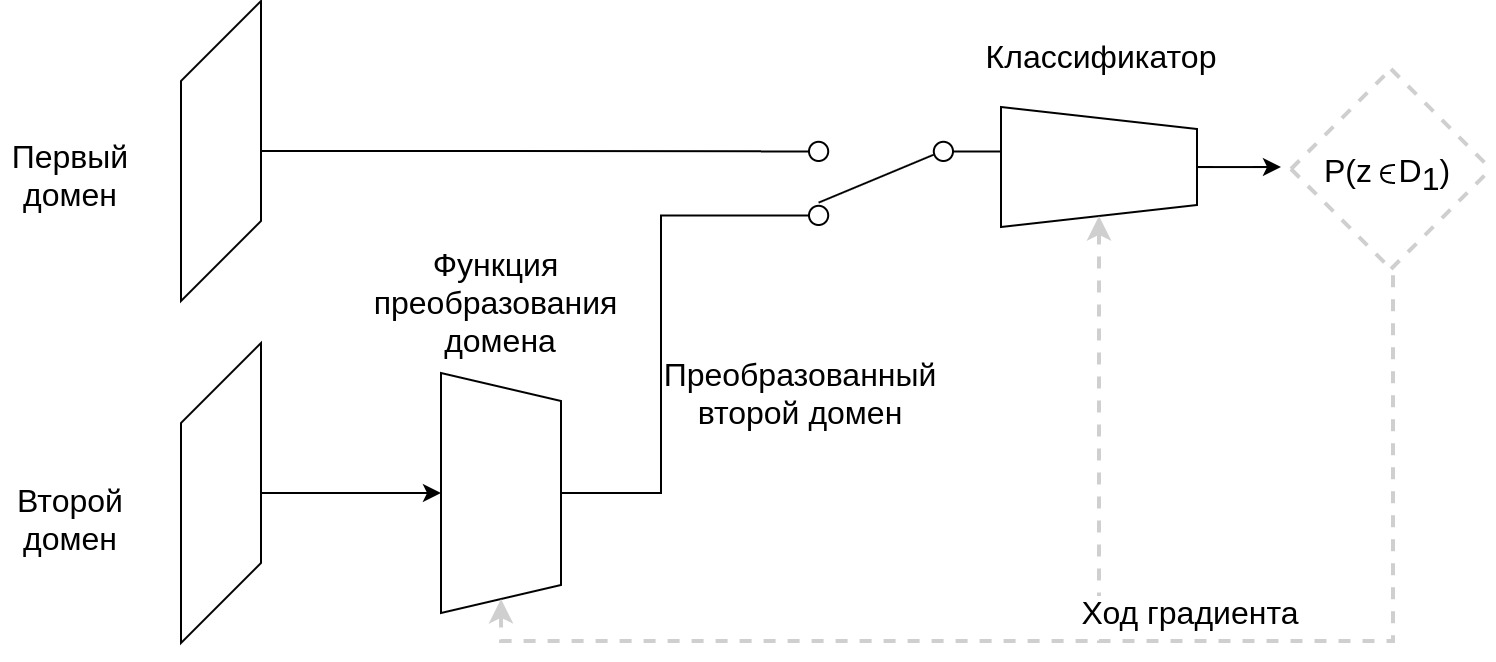
\includegraphics[width=0.7\textwidth]{pictures/new_model_schema.jpg}
    \caption{Предлагаемая архитектура модели для решения задачи нахождения параметров функции преобразования оптимальной относительно дивергенцией Кульбака-Лейблера}
    \label{fig_arch}
\end{figure}

С одной стороны, мы хотим, чтобы решения дискриминатора $D$ по данным из первого домена были точны, максимизируя $\expectation_{\bfx \sim g_1}[\log D(\bfx)]$. Между тем, учитывая преобразованную выборку второго домена $f(\bfz), \bfz\sim g_2$, ожидается, что дискриминатор покажет вероятность $D(f(\bfz))$, близкую к нулю, максимизируя $\expectation_{\bfz\sim g_2} [\log(1 - D(f(\bfz)))]$.

С другой стороны, генератор обучен увеличивать вероятность того, что $D$ даст высокую вероятность для преобразованного целевого домена, таким образом, чтобы минимизировать $\expectation_{\bfz\sim g_2} [\log(1 - D(f(\bfz)))]$.

При объединении обоих аспектов вместе получается, что $D$ и $f$ играют в минимаксную задачу, в которой мы должны оптимизировать следующую функцию потерь:

\begin{multline*}
    L_{KL}(D, f) =  \expectation_{\bfx\sim g_1}[\log D(\bfz)] + \expectation_{\bfz\sim g_2} [\log(1 - D(f(\bfz)))] = \\  \expectation_{\bfx \sim g_1}[\log D(\bfx)] + \expectation_{\bfx\sim f\circ g_2}[\log(1 - D(\bfx)]
\end{multline*}

где член $\expectation_{\bfx\sim g_1}[\log D(\bfx)]$ не влияет на $G$ во время обучения.

Итоговая оптимизационная задача:
\begin{equation}
    \label{minmax_for_KL}
    \min_f\max_D L_{KL}(D,f)
\end{equation}

% https://lilianweng.github.io/lil-log/2017/08/20/from-GAN-to-WGAN.html#kullbackleibler-and-jensenshannon-divergence

\newpage
\subsubsection{Постановка задачи для расстояния Васерштейна}

Теперь рассмотрим расстояние Васерштейна в качестве функции сходства. В общем случае расстояние Васерштейна имеет вид:

$$W_p(\mu, v) := \Big ( \inf_{\gamma \in \Gamma(\mu, v)} \int d(x, y)^p d\gamma(x, y) \Big)^{1/p}$$
где $\Gamma(\mu, v)$ обозначает совокупность всех мер с маргинальными распределениями $\mu$ и $v$ для первого и второго параметров соответственно.

Для оценки параметров функции преобразования будет использоваться расстояние Васерштейна-1 или Earth-Mover (EM) distance:

\begin{equation}
    \label{W1_intro}
    W(g_1, g_2) = \inf_{\gamma \in \Gamma(\mu, v)} \mathbb{E}_{(x, y) \sim \gamma} |x - y|
\end{equation}

$W$ также достигает минимума при совпадении распределений $g_1$ и $g_2$. 

% \textcolor{red}{\textbf{Вставить почему W - критерий!!!}}

Из \eqref{sim_funk_generated_by} получаем, что функция сходства порожденная расстоянием Васерштейна:
\begin{equation}
    \label{W_sim_function}
    s_{W} (g_1 , g_2) = \exp(-W(g_1 , g_2))
\end{equation}

Отметим, что с учетом \eqref{W_sim_function} задачу максимизации \eqref{opt_transorm_f} можно переписать в следующем виде:

$$\hat{\theta}_f = \argmin_{\theta_f} W ( g_1,  f\circ g_2)$$


Выражение \eqref{W1_intro} достаточно трудно вычислять, но с учетом, двойственности Канторовича-Рубинштейна \cite{Kantorovich_Rubinstein_duality}, которая говорит нам о том, что

\begin{equation}
    \label{w_supremum}
    W(g_1, g_2) = \sup_{\|D\|_L\leq 1} \expectation_{\bfx\sim g_1}[D(\bfx)] - \expectation_{\bfz\sim g_2}[D(\bfz)],
\end{equation}
где супремум берется по всеми 1-липшицевым функциям  $D : \bbr^n \to \bbr$. Причем, если мы заменим $\|D\|_L \leq 1$ на $\|D\|_L \leq K$, т.е. рассмотрим K-липшицевы функции для некоторой константы $K$, то получим $K \cdot W(g_1, g_2)$. Поэтому, если существует параметризованное семейство из функций $\{D_w\}_{w\in W}$, все из которых являются K-липшицевыми для некоторого K, то задача переписывается к задаче максимизации:

\begin{equation}
    \label{w_maximum}\max_{w \in W} \expectation_{\bfx\sim g_1}[D(\bfx)] - \expectation_{\bfz\sim g_2}[D(\bfz]
\end{equation}
Если супремум в \eqref{w_supremum} достигается для некоторого $w \in W$, то и максимум в \eqref{w_maximum} будет достигнут, его значение будет известно с точностью до мультипликативной константы. Однако важно, что данная константа не влияет на точку максимум, поэтому значения аргументов, в которых достигаются супремум и максимум будут совпадать.

Таким образом получается оптимизационная задача функции потерь:

$$L_W(f) = \max_{w \in W} \expectation_{\bfx\sim g_1}[D_w(\bfx)] - \expectation_{\bfz\sim g_2}[D(f(\bfz))]$$

Для нахождения параметров функции преобразования одного домена в другой оптимальной относительно расстояния Васерштейна решается оптимизационная задача:

\begin{equation}
    \label{minmax_for_W}
    \min_f L_{W}(f)
\end{equation}

\newpage
\section{Результаты экспериментов}

Цель эксперимента заключается в том, что мы хотим проверить верность гипотезы сформулированной в введении, и в том, что хотим определить, какая функция сходства позволяет достигать лучшие результаты. Хотим проверить верность утверждения, что полученная функция преобразования домена сохраняет инвариантность на классах и значениях целевых переменных. Для проведения эксперимента берется два различных домена и задача регрессии на первом из них. После этого находится оптимальная функция преобразования целевого домена в исходный и применяются два предлагаемых далее метода оценки качества функции преобразования.

Пусть функция преобразования сохраняет инвариантность на значениях целевых переменных, тогда:
\begin{enumerate}
    \item среднеквадратическое отклонение предсказываемого значения от правильного ответа на преобразованном целевом домене должно быть схоже с соответствующей величиной на исходном домене.
    \item можно статистически проверить гипотезу о равенстве весов в задачи линейной регрессии. Ожидается, что эта гипотезу будет неотвержима.
\end{enumerate}

В работе \cite{Aduenko_article} рассматривается задача различения моделей обученных на непересекающихся множествах. В ней выводится распределение значения функции сходства $s_0$ между апостериорными распределениями весов для пары линейных моделей в условиях истинности гипотезы $H_0$ о совпадении весов моделей. 

Пусть $\bfX_1$ и $\bfX_2$ есть выборки. Пусть тогда целевые переменные:

$$ \bfy_1 = \bfX_1\bfw_1 + \epsilon_1, \epsilon_1 \sim \mathcal{N} (0, \sigma^2_1\mathbf{I}), \bfw_1 \sim p_1(\bfw_1)$$
$$ \bfy_2 = \bfX_2\bfw_2 + \epsilon_2, \epsilon_2 \sim \mathcal{N} (0, \sigma^2_2\mathbf{I}), \bfw_2 \sim p_2(\bfw_2)$$
Считаем далее, что $p_1(\bfw_1)$ и $p_2(\bfw_2)$ есть нормальные распределения, то есть

$$ p_1(\bfw_1) = \mathcal{N} (\bfw_1|\bfv_1, \bsigma^{-1}_1), p_2(\bfw_2) = \mathcal{N} (\bfw_2|\bfv_2, \bsigma^{-1}_2).$$
Получаем, что функции совместного правдоподобия имеют вид

$$p(\bfy_k, \bfw_k|\bfX_k) = p(\bfy_k|\bfX_k, \bfw_k)p(\bfw_k) = \mathcal{N}(\bfy_k-\bfX_k\bfw_k|\mathbf{0}, \sigma^2_k\mathbf{I})\mathcal{N}(\bfw_k|\bfv_k, \bsigma^{-1}_k), \ k = 1, 2.$$
Пользуясь формулой Байеса, получаем для апостериорного распределения параметров $\bfw_1$ и $\bfw_2$ 

$$p(\bfw_k|\bfX_k, \bfy_k) = \frac{p(\bfy_k, \bfw_k|\bfX_k)}{p(\bfy_k|\bfX_k)} \propto p(\bfy_k, \bfw_k|\bfX_k), \ k = 1, 2,$$
откуда $p(\bfw_k|\bfX_k, \bfy_k) = \mathcal{N} (\bfw_k|\hat{\bfw}_k, \Tilde{\bsigma}^{-1}_k)$, где

$$\hat{\bfw}_k = \Big( \bsigma_k + \frac{1}{\sigma^2_k} \bfX^T_k\bfX_k\Big)^{-1} \Big( \bsigma_k\bfv_k + \frac{1}{\sigma^2_k}\bfX^T_k\bfy_k\Big)$$
есть оценка максимума апостериорной вероятности, а

$$\Tilde{\bsigma}_k = \bsigma_k + \frac{1}{\sigma^2_k}\bfX^T_k\bfX_k, \ k = 1, 2$$
Тогда для $s_0$ для пары апостериорных распределений имеем:

$$- 2 \log s_0 = (\hat{\bfw}_2 - \hat{\bfw}_1)^T \Bigg( \Big( \bsigma_1 + \frac{1}{\sigma^2_1}\bfX^T_1\bfX_1 \Big)^{-1} + \Big( \bsigma_2 + \frac{1}{\sigma^2_2}\bfX^T_2\bfX_2 \Big)^{-1} \Bigg)^{-1} (\hat{\bfw}_2 - \hat{\bfw}_1).$$
И также выводится, что $-2 \log s_0 \xrightarrow{d} \chi^2(n)$.

\newpage
\subsection{Вычислительный эксперимент для отзывов с сайта Amazon}

Вычислительный эксперимент проводился на данных об отзывах о товарах с сайта Amazon. Домену соответствовала категория, и строилось векторное представление для каждого отзыва. Также каждому отзыву соответствует оценка, которую поставил пользователь. В качестве различных доменов были взяты категории "Industrial and Scientific"(I\&S) и "Luxury Beauty"(LB)

Находились две функции преобразования домена LB в I\&S по дивергенции Кульбака-Лейблера и по метрики Васерштейна. Вследствие двух теорем выше функция сходства Адуенко в вычислительном эксперименте не участвовала. Для каждой из построенных функций преобразования обучалась модель регрессии оценки пользователя.

\begin{figure}[H]
        \centering
        \subfloat[\centering ]{{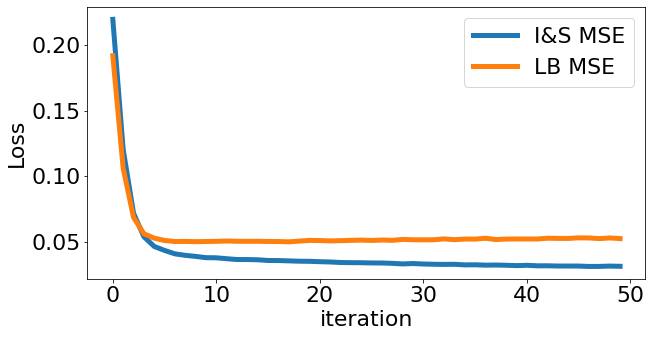
\includegraphics[width=0.5\textwidth]{pictures/texts_KL_regres.png} }}
        \qquad
        \subfloat[\centering ]{{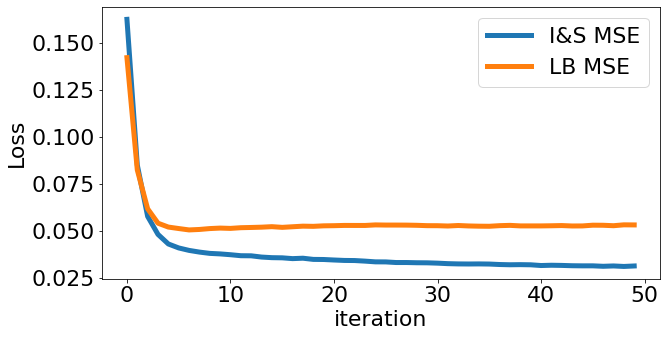
\includegraphics[width=0.5\textwidth]{pictures/texts_Wass_regres.png} }}
        
        \caption{Среднеквадратическое отклонение предсказываемого значения от правильного ответа для (a) дивергенции Кульбака-Лейблера и (b) для расстояния Васерштейна, результаты весьма схожи.}
        % \label{example:1}
    \end{figure}

\begin{table}[H]
    \centering
    \begin{tabular}{||c|c|c||}
        \hline 
         & Дивергенция Кульбака-Лейблера & Расстояние Васерштейна \\
        \hline\hline
        p-value & 0.1311 & 0.3412 \\
        \hline
    \end{tabular}
    \caption{Статистическая проверка гипотезы о равенстве весов в задаче линейной регрессии на домене I\&S и преобразованном домене LB для различных функций преобразования оптимальных относительно дивергенции Кульбака-Лейблера и расстояния Васерштейна соответственно.}
    \label{tab:my_label}
\end{table}



\subsection{Вычислительный эксперимент для бинаризованных изображений фигур}

Данный вычислительный эксперимент проводился на бинаризованных изображениях. Были взяты два домена~--- изображения с различными фигурами. Первому соответствовали квадраты, второму круги. Каждой фигуре можно задать в соответствие координаты центра фигуры и ее радиус.

Как и раньше, находились функции преобразования доменов по дивергенции Кульбака-Лейблера и по метрики Васерштейна. Для каждой из построенных функций преобразования обучалась модель регрессии радиуса фигуры.

\newpage 

\thispagestyle{empty}
\begin{figure}[H]
        \centering
        \subfloat[\centering ]{{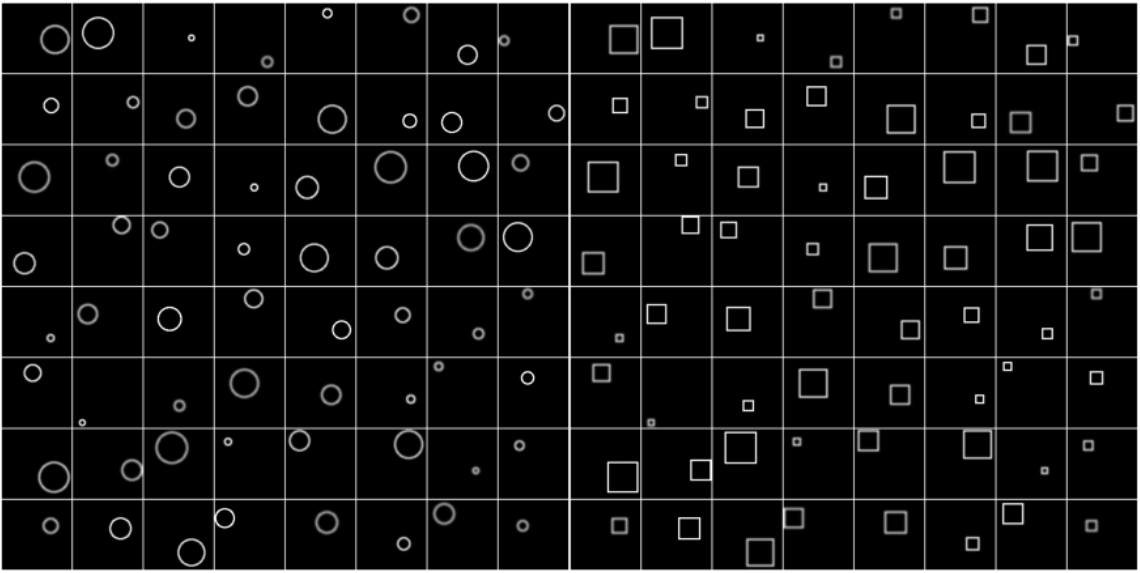
\includegraphics[width=0.8\textwidth]{pictures/original_images.png} }}
        \qquad
        \subfloat[\centering ]{{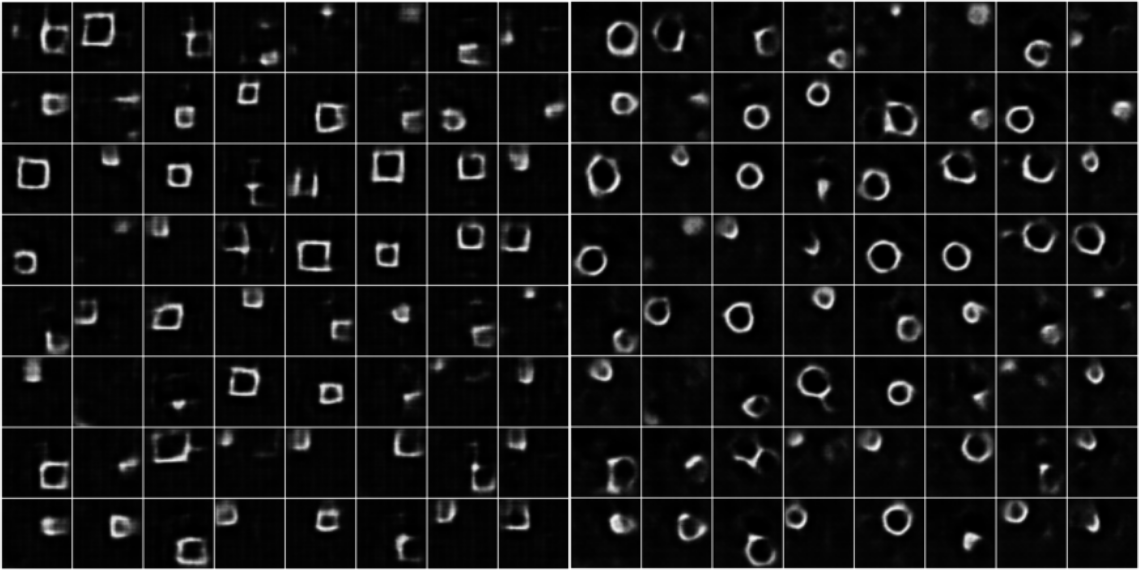
\includegraphics[width=0.8\textwidth]{pictures/transformed_KL.png} }}
        \qquad
        \subfloat[\centering ]{{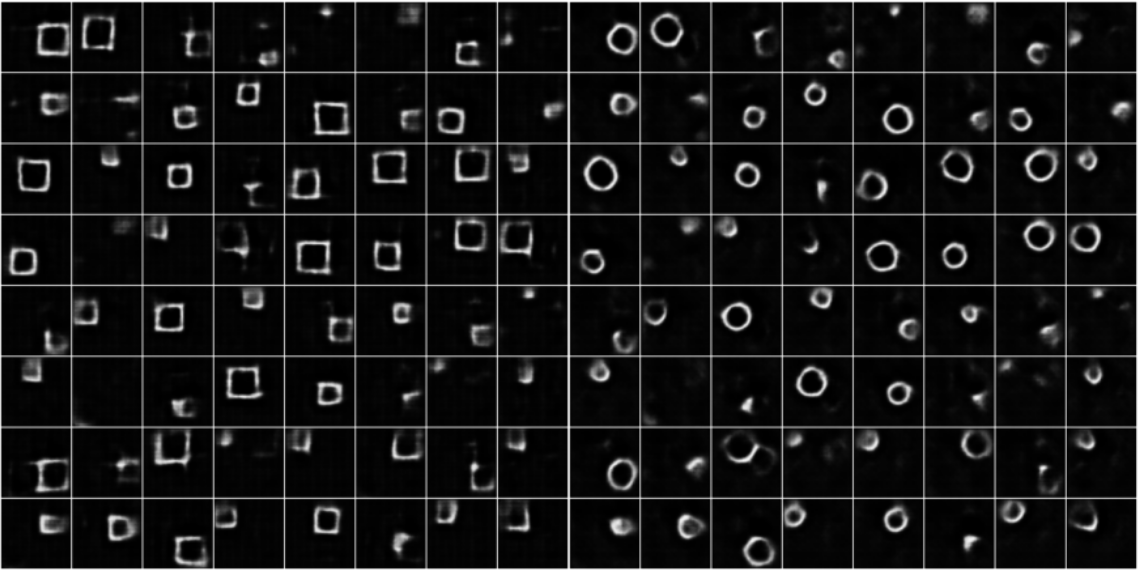
\includegraphics[width=0.8\textwidth]{pictures/transformed_Wass.png} }}
        
        \caption{(a) оригинальные изображения. Изображения преобразованные с помощью (b) дивергенции Кульбака-Лейблера или (c) расстояния Васерштейна. Важно отметить, что при применении функции преобразования фигура меняла форму, но не положение или размер.}
        % \label{example:1}
    \end{figure}

\begin{figure}[H]
    \centering
    \subfloat[\centering ]{{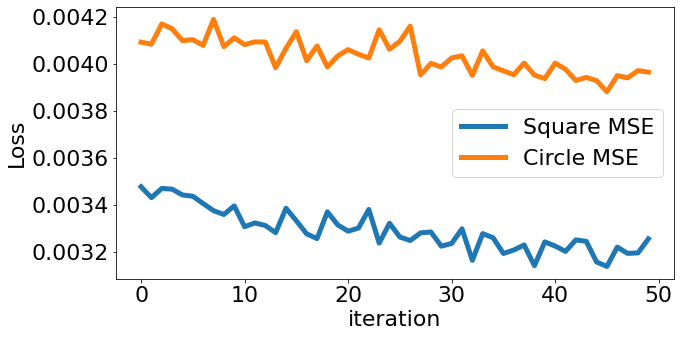
\includegraphics[width=0.5\textwidth]{pictures/images_KL_regres.png} }}
    \qquad
    \subfloat[\centering ]{{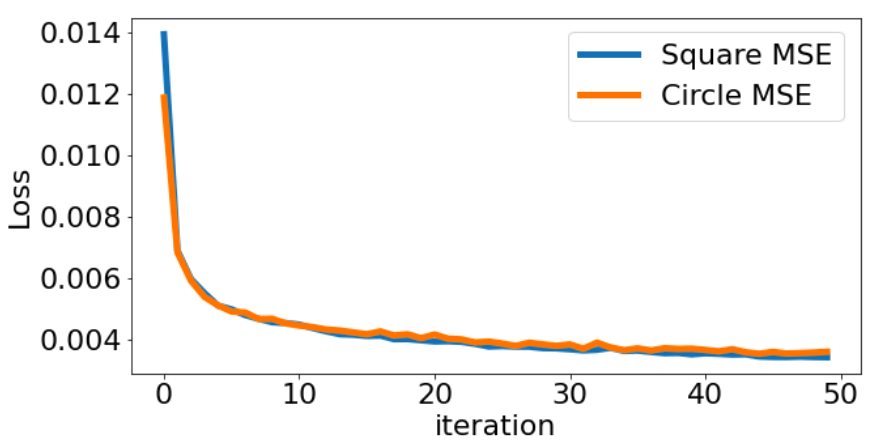
\includegraphics[width=0.5\textwidth]{pictures/images_Wass_regres.png} }}
    
    \caption{Среднеквадратическое отклонение предсказываемого значения от правильного ответа для (a) дивергенции Кульбака-Лейблера и (b) для расстояния Васерштейна.}
    % \label{example:1}
\end{figure}

\begin{table}[H]
    \centering
    \begin{tabular}{||c|c|c||}
        \hline 
         & Дивергенция Кульбака-Лейблера & Расстояние Васерштейна \\
        \hline\hline
        p-value квадрат в круг & 0.1682 & 0.2994 \\
        \hline
        p-value круг в квадрат & 0.1778 & 0.2620 \\
        \hline
    \end{tabular}
    \caption{Статистическая проверка гипотезы о равенстве весов в задаче линейной регрессии для бинаризованных картинок фигур.}
    \label{tab:my_label}
\end{table}

\newpage
\section{Заключение}

В работе предложен метод решения задачи доменной адаптации через оценку параметров функции преобразования домена. Теоретически доказано, что функция сходства предложенная Адуенко А.\ А. не является достаточным условием совпадения распределений. По этой причине она не может использоваться для оценки параметров функции преобразования. Также описан алгоритм нахождения функции преобразования, оптимальной относительно дивергенции Кульбака-Лейблера и расстояния Васерштейна.

В ходе вычислительного эксперимента подтверждена гипотеза о том, что функция преобразования сохраняет инвариантность на классах и значениях целевых переменных. Также было установлено, что расстояние Васерштейна позволяет строить более качественную функцию преобразования. Хотя достигаемое среднеквадратическое отклонение ведет себя одинаково, но второй тест, который заключается в статистической проверке равенства весов моделей линейной регрессии показывает преимущество использования расстояния Васерштейна.

% \section{Дополнение}


\addcontentsline{toc}{section}{\protect\numberline{}Список литературы}

\begin{thebibliography}{99}

\bibitem{DANN}
    \BibAuthor{Yaroslav Ganin and Evgeniya Ustinova and Hana Ajakan and Pascal Germain and Hugo Larochelle and François Laviolette and Mario Marchand and Victor Lempitsky}.
    \BibTitle{Domain-Adversarial Training of Neural Networks}, 2016 

\bibitem{ADDA}
    \BibAuthor{Eric Tzeng and Judy Hoffman and Kate Saenko and Trevor Darrell}.
    \BibTitle{Adversarial Discriminative Domain Adaptation}, 2017

\bibitem{M-ADDA}
    \BibAuthor{Issam Laradji and Reza Babanezhad}.
    \BibTitle{M-ADDA: Unsupervised Domain Adaptation with Deep Metric Learning}, 2018
    
\bibitem{saito2018maximum}
    \BibAuthor{Kuniaki Saito and Kohei Watanabe and Yoshitaka Ushiku and Tatsuya Harada}.
    \BibTitle{Maximum Classifier Discrepancy for Unsupervised Domain Adaptation}, 2018

\bibitem{shu2018dirtt}
    \BibAuthor{Rui Shu and Hung H. Bui and Hirokazu Narui and Stefano Ermon}.
    \BibTitle{A DIRT-T Approach to Unsupervised Domain Adaptation}, 2018

\bibitem{Aduenko_article}
    \BibAuthor{А.А.~Адуенко}.
    \BibTitle{Выбор мультимоделей в задачах классификации}, 2017 

\bibitem{GAN_article}
    \BibAuthor{Ian J. Goodfellow and Jean Pouget-Abadie and Mehdi Mirza and Bing Xu and David Warde-Farley and Sherjil Ozair and Aaron Courville and Yoshua Bengio}.
    \BibTitle{Generative Adversarial Networks}, 2014

\bibitem{Kantorovich_Rubinstein_duality}
    \BibAuthor{C´edric Villani}. 
    \BibTitle{Optimal Transport: Old and New}. Grundlehren der mathematischen Wissenschaften. Springer, Berlin, 2009.


\end{thebibliography}


\end{document}